\section{Skill Maintenance}

Managing Skills
\newline\newline
Within murcS it is very easy to manage skills. Skills main purpose is to give an idea of what individual people are experienced in. Skills should be generic so that they can be added to multiple people. Some examples might be C\#, Java, Python, Talking.
\newline
When you wish to create a new skills simply go to the display list and select skills. Then following the same process as People, Teams etc. either click the add button in the bottom of the list or select File/New/Skill. Once you have done this a creation dialog will appear as shown below.

\begin{figure}[H]
\centering
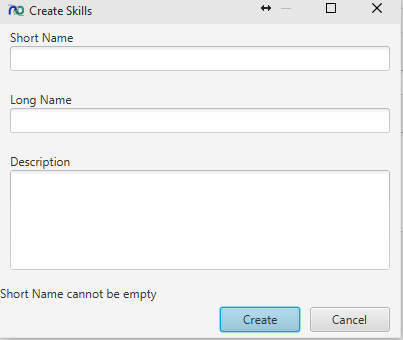
\includegraphics[width=\textwidth]{images/screenshots/skills1.PNG}
\caption{Creating a Skill}
\label{fig:new_project}
\end{figure}

When you create a skill the only compulsory field is the short name, this should be along the lines of C\# or Java. The long name is optional and could be for example C Sharp. The description should just detail what the skill means in particular.
\newline\newline
When you've created a skill you can then edit them and delete them in a very similar way to teams and people. Simply select the skill you want to edit or delete and then either edit it in the edit pane that appears in the main screen or click the delete button at the bottom of the display list. If you are deleting the skill it will tell you where the skill is used and if you still want to delete the skill it will delete it from all of the people it was linked with. The only skills that are not deletable are PO and SM as theses are necessary for Scrum.